\documentclass[conference]{IEEEtran}

  \usepackage{booktabs}
  \usepackage{listing}
  \usepackage{amsmath}
  \usepackage{algorithm}
  \usepackage{array}
  \usepackage{url}
  \usepackage{cite}
  \usepackage{complexity}
  \usepackage{algpseudocode}
   \usepackage{graphicx}
   \usepackage{enumerate}
% \usepackage{algorithm}
  \ifCLASSINFOpdf
  
  \else
  
  \fi
  
  \hyphenation{op-tical net-works semi-conduc-tor}
  
  
  \begin{document}
  
  \title{Parallel Distributed Multi-objective Fuzzy Genetics-based Machine Learning \\ Mid Term Report}
  
  \author{\IEEEauthorblockN{Bowen Zheng, Shijie Chen, Shuxin Wang}
  \IEEEauthorblockA{Department of Computer Science and Engineering\\
  Southern University of Science and Technology\\
  Shenzhen, Guangdong, China\\}
  }
  
  \maketitle
  
  \begin{abstract}
  In the second period of the project, we finished the design of fuzzy classifiers, GBML framework and the asynchronous parallel distributed system. We have implemented each part respectively and are working to integrate them together.
  \end{abstract}
  \IEEEpeerreviewmaketitle
  
  \section{Introduction}
  In this project, we aim to build a parallel distributed implementation of a multi-objective genetics based machine learning(GBML) algorithm. We choose a specific problem of a three-objective fuzzy rule-based classifier and fit it into a hybrid GBML framework. Then we develop a parallel mechanism to accelerate computation.

  Code of the three parts have been completed. We will integrate them together, fix bugs and run some test problems in the next stage.

  \section{Fuzzy Rule-based Classifiers}
  The design and implementation of fuzzy classifier is based on \cite{ishibuchi2007analysis}.
  \subsection{Fuzzy Rules}
  \subsection{Fuzzy Classifier}

  \section{Hybrid Genetics-based Machine Learning Framework}
	 \par After designing the fuzzy classifier, the next step is approaching our three objectives: correctly classified training patterns, number of fuzzy rules and total number of antecedent conditions in the fuzzy classifier S. Currently we only implement the two objects.
	 \par
	 We use a hybrid GBML algorithm to find the non-dominated rule sets of this problem. The genetic algorithm we used is basically following \cite{ISHIBUCHI20074}. This hybrid GBML is implemented in the framework of non-dominated sorting genetic algorithm II(NSGA-II) and it's a Pittsburgh-style algorithm. Besides, it use Michigan-style GBML to change a rule as the mutation operation. 
	 \par
	In our genetic algorithm, the population is a set of fuzzy classifier, and the individual is a single fuzzy classifier (i.e., a set of fuzzy rules). The basic steps of our algorithm is followed. First step, we'll initialize our population with size $N_pop$ using training data. Second step, we'll generate $N_pop$ offspring by implementing selecting and crossover operators to two parents, and do mutate on the offspring. Third step, the origin and offspring population will be combined together and we only keep the first $N_pop$ individuals after the population sorting by Pareto ranking and crowding measure, which will be introduced later. Finally, we'll check whether it have reached the stop condition,and if not we'll go back to the second step.
	 
	 \subsection{NSGA-II}
	 \par
	 NSGA-II is introduced detailedly in \cite{996017}, which is a common algorithm in multi-objective optimizing problem. I think the characters of NSGA-II algorithm comparing with a ordinary genetic algorithm is that it uses elite-preserving, Pareto ranking, and crowding measure. Elite-preserving is a strategy that can reserve outstanding gene by keeping the individual containing such a gene. Pareto ranking and crowding measure is used to compare individuals in the three-objective situation. We'll introduce the three futures respectively.
	 \subsubsection{Elite-preserving}
	 \par
	 Elite-preserving is a replacing strategy at the end of a generation. The basic idea is that we only replace individuals with bad performance in original population by the outstanding offspring, and we keep preeminent parents to reserve their high performance gene. And we measure individuals' performances using Pareto ranking and crowding measure.
	 
	 
	 \subsubsection{Pareto ranking}
	 \par
	 Pareto-optimal front is the solution set that we want to find in the multi-objective optimizing problem, and its definition can been seen at \cite{ISHIBUCHI20074}. In the multi-objective optimizing problem, individual in Pareto-optimal front can be seen as the "best" solution. We'll give these individuals the highest Pareto ranking. If we remove the individuals in Pareto-optimal front, we can find another Pareto-optimal front of the remaining individuals. Then we'll give the second front a lower Pareto ranking than previous one, and we continue do such iteration until every individual gets their Pareto ranking. And we can measure individuals' performance by their Pareto ranking. If individuals have same ranking number, we'll compare them by using crowding measure.
	 
	 \subsubsection{Crowding measure}
	 \par
	 Crowding measure can help us finding a more diverse Pareto set. As we wanting to find a more homogeneous solutions set, we'd like to choose the individual in a less crowded area. To estimate the density of a individual in a population, we calculate the sum of the distances to neighbor individuals on both side and for each objective. And shorter the distance is, more crowded area the individual is in.     
	 
	 \subsection{Michigan-style GBML}
	 \par
	 Different Pittsburgh-style algorithm, Michigan-style GBML see a single fuzzy rule as a population and see the membership function as an individual. So we use Michigan-style GBML as a mutation operator acting on a single rule to enrich the diversity of our population. 
	 \subsection{Validation}
	 After implementing our program, we validate its reliability using iris data set and it have successfully pass the feasibility test. The results are followed.
	 \\
	 \begin{tabular}{cccccc}
	 	\hline
	 	Number of rules& 1& 2&3&4&5\\
	 	\hline
	 	NO. of correctly classified pattern& 49& 99&132&134&137\\
	 	\hline
	 	error rate&0.67&0.34&0.12&0.11&0.09\\
	 	\hline
	 \end{tabular}

 \begin{figure}[H]
 	\centering
 	\includegraphics[width=0.5\textwidth]{iris.png}
 	\caption{Result on iris data set}\label{fig:digit1}
 \end{figure}
  \section{Asynchronous Parallel Distributed System Design}
We propose a new asynchronous parallel distributed model to reduce the cost of time on our fuzzy classifier GBML (Fig.\ref{fig:digit2} Fig.\ref{fig:digit3}). Our model can be represented as 3 parts: 1. Dataset distributor 2. Local island worker model 3. Population migration control. (For convenience, slave process will be called as island)

 \begin{figure}[H]
	\centering
	\includegraphics[width=0.5\textwidth]{master.png}
	\caption{Master process}\label{fig:digit2}
\end{figure}
\begin{figure}[H]
	\centering
	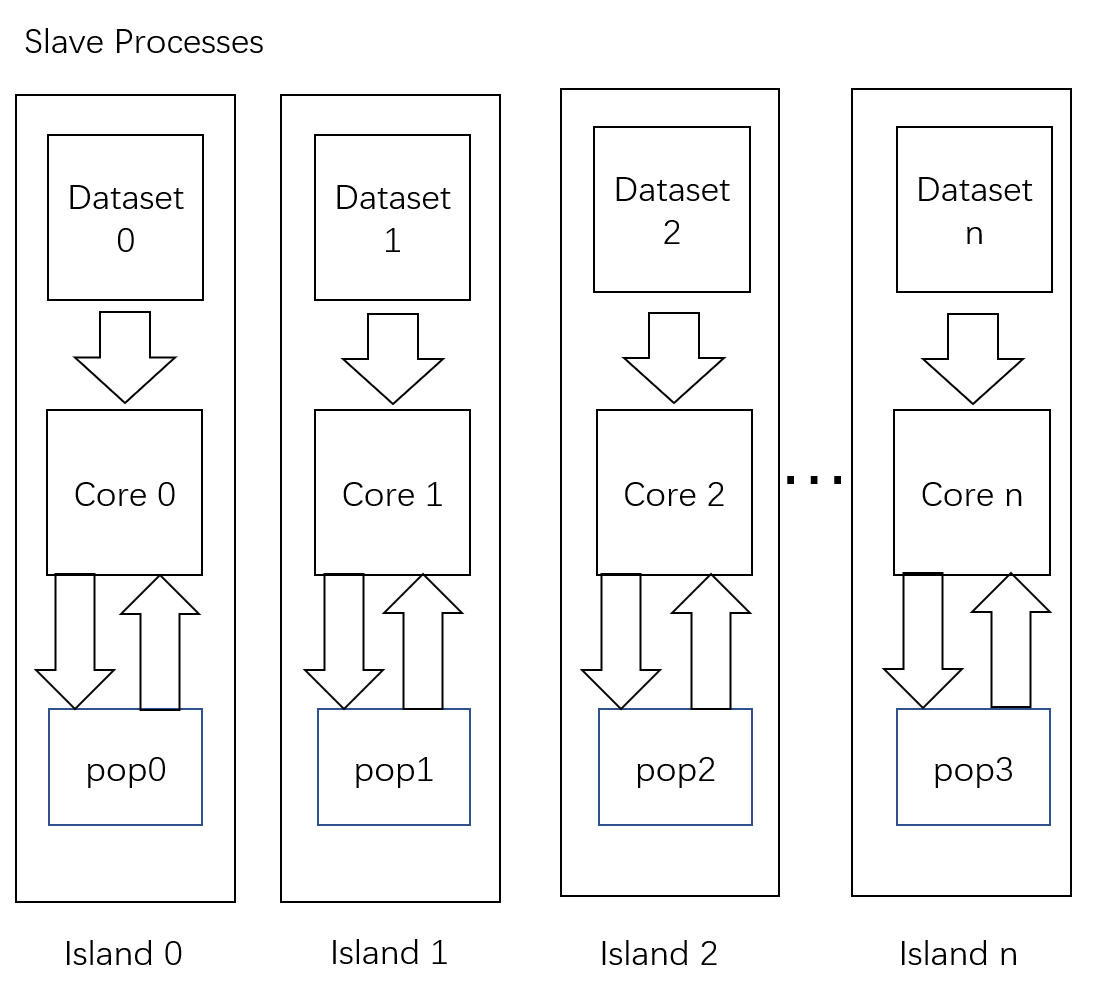
\includegraphics[width=0.5\textwidth]{slave.png}
	\caption{Slave processes}\label{fig:digit3}
\end{figure}

	\subsection{Main Algorithm:}
		\subsubsection{Master Process:}	
		\begin{enumerate}[(i)]
			\item read dataset and initialize the dataset pool 
			\item distribute $N_{land}$ simples to each P islands through dataset distributor layer.
			\item start P slave processes, which each of them works on a cpu core.
			\item wait for all islands run its “init” part and return their population. Use these populations, build an initialized population pool.
			\item generate new population for each island and start its "main" part
			\item Lisening each island, exchange(migrate) population when an island run a certain iterations $I_{update}$.
			\item terminate when all listener recerive the stop message.
		\end{enumerate}

		\subsubsection{Slave Process:}
			\begin{enumerate}[(i)]
				\item init:
				\begin{enumerate}[(1)]
					\item reveive the dataset from the master process and store it.
					\item initial population from the dataset.
					\item run the GBML with $I_{init}$ iterations.
					\item upload the roughly trained population to the master process.
				\end{enumerate}
				\item main:	
				\begin{enumerate}[(1)]
					\item run the GBML with $I_{update}$ iterations.
					\item upload the population to the master process and wait for the new population from the master process population migration control layer.
					\item check the termination condition, if the condition reaches, send a stop message to the master process.
					Otherwise repeat procedures "main" (1),(2).
					
									
				\end{enumerate}
			\end{enumerate}



	\subsection{Dataset distributor:}
	This layer is responsible for the dataset distribution process, which delivering a partial of dataset to each island. During this process, the distributor picks $N_{land}$ data from the dataset pool without replacement, then put them into an island on one slave process. Repeat this procedure until all islands get their “environment”
	\subsection{Migration Algorithm:}
	This layer is responsible for the population exchange process. Before slave processes run “init” part, this layer establishes connections between the master process and each other island to listen to them. When an island completes that part, it will stop, upload the current population to this layer and wait for new population feedback from this layer. After this layer receives roughly trained population from all islands, it will generate a population pool based on these population and finished the initialization of this layer.
	
	
	After the initialization, this layer will delivering new population to each island and start their “main” part. The new population is generated by random sampling $ N_{pop_i}$ individuals from the population pool without replacement.
	
	
	After the “main” part is started, each island can choose to update its population through this layer when finished certain iterations $I_{update}$ by themselves, which is known as one epoch.This layer will firstly put the population uploaded from the island to the pool and randomly select the same amount of individual from the pool, then delete them from the pool. Note that comparing to the process of initialization of population pool, the control rule is given to the island rather than this control layer, therefore it is a more asynchronous way to deal with the migration of population between the island and the big population pool, which will reduce or even eliminate the barrier time cost. This will significantly improve the performance when the spent time on each epoch varies dramatically for different islands.
	
  \section{Contribution}
  
    \begin{itemize}
    \item Bowen Zheng - Design \& Implementation of parallel system
    \item Shijie Chen - Design \& Implementation of fuzzy classifier, Design of parallel system
    \item Shuxin Wang - Design \& Implementation of Hybrid GBML framework
    \end{itemize}
    

  \section*{Acknowledgment}


\bibliographystyle{ieeetr}
\bibliography{ref}
% that's all folks
\end{document}


  